\documentclass[border=10pt]{standalone}
\usepackage[T1]{fontenc}
\usepackage[siunitx, RPvoltages]{circuitikz}
\ctikzset{logic ports=ieee}
\tikzset{small buffer/.style={%
		ieeestd buffer port, /tikz/circuitikz/logic ports/scale=.8},
	small inline not/.style={%
		inline not, /tikz/circuitikz/logic ports/scale=0.8}
}
\begin{document}
	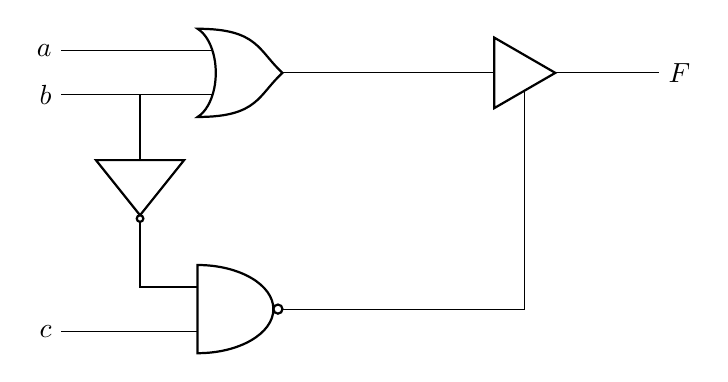
\begin{tikzpicture}[]
		\node[nand port] (nand0) at (0,0) {};
		\node[or   port] (or0)   at (0,3) {};
		\node[small buffer] (tri0) at (3,3) {};
		
		\draw (or0.in 2) -- ++(-.5,0)
		to[small inline not] ($(nand0.in 1) + (-.5,0)$)
		-- (nand0.in 1);
		
		\draw (or0.in 1)   -- ++(-1.5,0) node[left] {$a$};
		\draw (or0.in 2)   -- ++(-1.5,0) node[left] {$b$};
		\draw (nand0.in 2) -- ++(-1.5,0) node[left] {$c$};
		
		\draw (tri0.in 1) -- (or0.out);
		\draw (tri0.out) -- ++(1,0) node[right] {$F$};
		\draw (tri0.down) |- (nand0.out);
	\end{tikzpicture}
\end{document}